\appendix



\section{Appendix A - Matlab Code}
\label{sec:Appendix A}
\begin{subappendices}
\subsection{Part 5.1}
\lstinputlisting{../MATLAB/scripts/p1.m}
\subsection{Part 5.2}
\lstinputlisting{../MATLAB/scripts/p2.m}
\lstinputlisting{../MATLAB/scripts/PSD_psi_omega.m}
\subsection{Part 5.3}
\lstinputlisting{../MATLAB/scripts/p3.m}
\subsection{Part 5.4}
\lstinputlisting{../MATLAB/scripts/p4.m}
\subsection{Part 5.5}
\lstinputlisting{../MATLAB/scripts/p5.m}
\end{subappendices}

\section{Appendix B - Simulink Diagrams}
\begin{subappendices}
\subsection{Part 5.1}
\begin{figure}
\caption{Model for Part 5.1 - Tunable parameter set in MATLAB for either sine wave (part b, c) or step function (part d) inputs.}
	\centering
		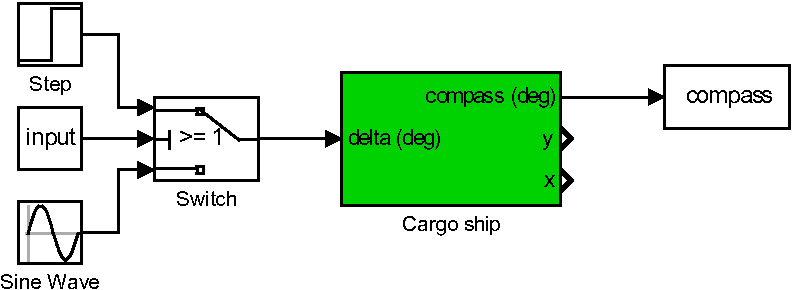
\includegraphics{images/ship_p1.pdf}
	\label{fig:ship_p1}
\end{figure}


\subsection{Part 5.3}
\begin{figure}
\caption{Model for Part 5.3 - Top Level - PD Controller takes a setpoint and compass measurement feedback as inputs and returns a rudder input as an output.}
	\centering
		\includegraphics{images/ship_p3_main.pdf}
	\label{fig:ship_p3_main}
\end{figure}


\begin{figure}
\caption{Model for Part 5.3 - PD Controller - Calculates error, Converts to Radians, Multiplies by Gain, Send through Transfer Function, Converts back to Degrees and clamps the output}
	\centering
		\includegraphics{images/ship_p3_PDController.pdf}
	\label{fig:ship_p3_PDController}
\end{figure}



\subsection{Part 5.5}

\end{subappendices}
